\documentclass{beamer}

\usepackage[utf8]{inputenc}
\usepackage{default}
\usepackage{multicol}
\usetheme{Warsaw}
\usecolortheme{seahorse}
\useoutertheme{shadow}
\useinnertheme{rectangles}

\title[Fibonacci Heap]{Fibonacci Heap}
\author[ALMA\and *Alexis\and Luis \and Margarita \and Ademir*]{{Bernal Chauayo, Luis Antonio}\\{Lacuaña Apaza, Margarita}\\{Mendoza Villarroel, Alexis}\\{Villena Zevallos, Ademir}}
\institute{{Ciencia de la Computación}
\\{Universidad Nacional de San Agustin}}
\date{2 de Octubre del 2016}

\begin{document}

\begin{frame}[plain]
    \titlepage
 \end{frame}
  
 \begin{frame}
  \frametitle{Índice}
  \begin{multicols}{2}
  \tableofcontents
  \end{multicols} 
\end{frame}

\section{Historia}

\begin{frame}
    \frametitle{Historia}
 \begin{itemize}
    \item Los Fibonacci heap  fueron desarrollados en 1984 por Michael L. Fredman y Robert E. Tarjan.
    \item Publicados por primera vez en una revista científica en 1987.
    \item El nombre de montículos de Fibonacci viene de la sucesión de Fibonacci, que se usa en pruebas comparativas de tiempo (Benchmarking).
\end{itemize}
\end{frame}

\section{Insertar}
\begin{frame}
  \frametitle{Insertar}
  \begin{columns}[t]
    \column{0.5\textwidth}
    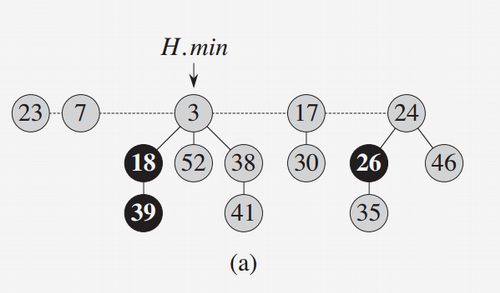
\includegraphics[width =1 \textwidth]{imagenes/insertar1.png}
      
    \column{0.5\textwidth}
    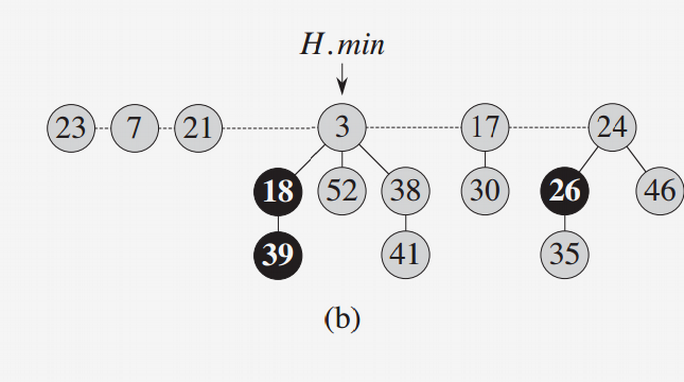
\includegraphics[width =1 \textwidth]{imagenes/insertar2.png}

   \end{columns}
  
  
\end{frame}
  
\end{document}
